\documentclass[11pt,a4paper,titlepage]{article}
\usepackage{graphicx}
\usepackage[margin=1in]{geometry}
%\usepackage{titling}
\usepackage{booktabs}
\usepackage[hidelinks]{hyperref}
\usepackage{float}


\usepackage{epstopdf}

\DeclareGraphicsExtensions{.png}
\DeclareGraphicsExtensions{.jpg}
%\DeclareGraphicsExtensions{.eps}

\begin{document}
\begin{titlepage}
	\begin{center}
		
		\begin{figure}[t]
			\centering
			
\includegraphics[width=350px]{UP_Logo.png}
		\end{figure}		
	
	
	\begin{flushright} 
		
		\textbf{\LARGE COS 301 Main Project}
		\newline \newline \newline
		\textbf{\LARGE Requirements and Design Specifications}
		\newline \newline \newline
 		\textbf{\LARGE ThinkTech}
		\newline \newline \newline
	\end{flushright}
		
		\vspace{1 cm}
		
		\LARGE{\textbf{Group Members: }}
		
		%\begin{minipage}{0.4\textwidth}

		\begin{flushright} \large
			Lelethu Zazaza 13028023\newline
			Goodness Adegbenro 13046412\newline
		\end{flushright}
		%\end{minipage}
		
	
		
		\textbf{Git repository link:\\}
		 \url{ https://github.com/COS301-ThinkTech}
		
		\vfill
		
		{\LARGE Version 0.1}
		\\
		{\large \today}		
		
		
	\end{center}
\end{titlepage}


\newpage
\tableofcontents


\pagebreak

\section{Vision and scope}
\subsection{Project background}
The flowchart planning and simulation  tool is a visual tool which aims to introduce programming logic to students by providing  a platform to construct  and execute  flowcharts which depict basic programming structures whilst validating whether the flowchart components are valid .

\subsection{Project vision}

Most first year computer science students come from a backgroud void of programming to a programming backgroud 
and they struggle to grasp the logical programming concepts quickly and easily.
Therefore, this project sets out to create an application with a simplified and easy-to-use interface for the planning and simulation of flowcharts, which
can be used in an education setting for an introductory program logic course. The objective is to
develop an application that can feasibly be used in such a practical setting. The application must be
visual in nature, due to the visual nature of flowcharts. The application must facilitate exploration
and experimentation, while providing clear feedback to the user as to how the program executes.

\subsection{Project scope}

The project consists of the following two components:

\begin{itemize}
\item A planning canvas, in which a flowchart can be built using an intuitive drag-and-drop editor.
Flowchart components will be selected and dropped into the canvas, and connected into
complete flowcharts. The system will also have to do error checking on the constructed
flowcharts, so that (for example) multiple entry points into a program or certain flowchart
components are not allowed.
\item An execution system, in which a flowchart can be run from start to finish. The system
should allow for one-click execution of the entire program, as well as step-by-step
execution. At all stages during execution, the currently executing component should be
highlighted, as well as the connection path being followed. The program's execution should
be very visually apparent and appealing. The output of the flowchart's execution should also
be apparent.
\end{itemize}

The following components are specifically excluded from the scope of the project:

\begin{itemize}
\item No executable program code generation will be required for this project.
\item No complex design elements (such as user-defined component assemblies) are required.
Only the basic components of standard flowcharts are necessary.\\

\end{itemize}

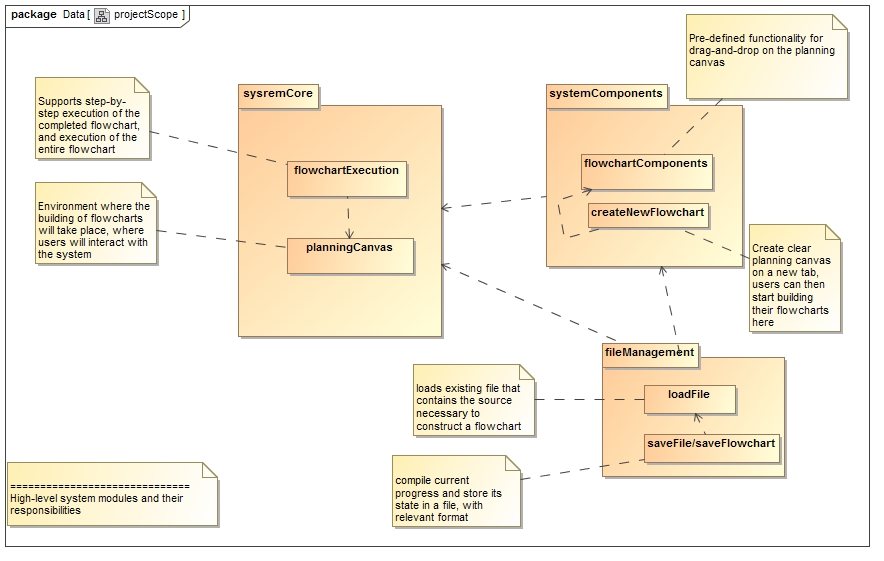
\includegraphics[width=500px]{projectScope.jpg}
\centerline{High level system modules and their responsibilities.}
% Include auxillary files here:  \input{file} 


\newpage	
\section{Use case prioritization}


\begin{table}[h!]  
    \caption{Use case prioritization}
    \label{tab:table1}
    \begin{tabular}{ccc}
      \toprule
      Critical & Important & Nice-To-Have\\
      \midrule	
      createFlowchartProject & addFlowchartComponent &  drag-and-drop flowchart into bin\\
      deleteFlowchart & editFlowchartComponent & \\
       & deleteFlowchartComponent & \\
       & saveFlowchart & \\
       & loadFlowchart & \\
       & runSimulationTool & \\
      \bottomrule
    \end{tabular}  
\end{table}


\newpage
\section{Use cases}

\subsection{createFlowchartProject}
Creates an environment to enable users to start building flowcharts.\newline\newline
\textbf{Pre Condition:} Planning canvas must be blank.\newline\newline
\textbf{Post Condition:} New canvas with Start and Return component created.\newline
\textbf{Post Condition:} Flowchart tools ready for use\newline

\begin{figure}[H]
  \centering
\includegraphics[width=500px]{createNewFlowchartProject.eps}
\caption{createFlowchartProject Use Case Diagram}
\end{figure}

\begin{figure}[H]
  \centering
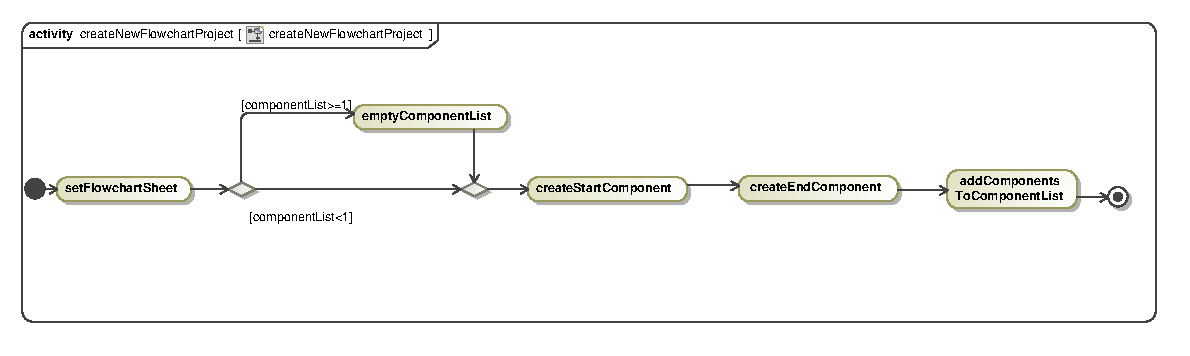
\includegraphics[width=500px]{createNewFlowchartProjectActivity.eps}
\caption{createFlowchartProject Activity Diagram}
\end{figure}

\newpage
\subsection{addFlowchartComponent}

Provides users with functionality to select the flowchart components they want to add and place it on the planning canvas.\newline\newline
\textbf{Pre Condition:} Canvas is available and flowchart exist.\newline\newline
\textbf{Post Condition:} Component has been added to flowchart and appers on canvas with the necessary connections, if any.

\begin{figure}[H]
  \centering
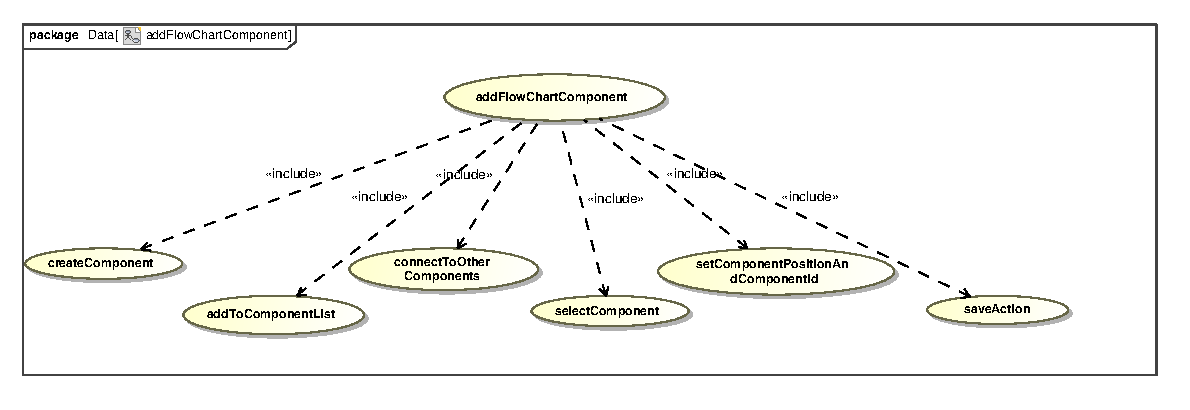
\includegraphics[width=500px]{addFlowChartComponent.eps}
\caption{addFlowchartComponent Use Case Diagram}
\end{figure}

\begin{figure}[H]
  \centering

\includegraphics[width=200px]{figure.jpg}
\caption{addFlowchartComponent Activity Diagram}
\end{figure}

\newpage
\subsection{editFlowchartComponent}

The editFlowchartComponent use case provides functionality for the user to edit each component of the flowchart on the canvas \newline\newline
\textbf{Pre Condition:} Component must have been added to the canvas\newline\newline
\textbf{Post Condition:} Component has been edited and saved\newline
\textbf{Post Condition:} Edited component has been saved

\begin{figure}[H]
  \centering
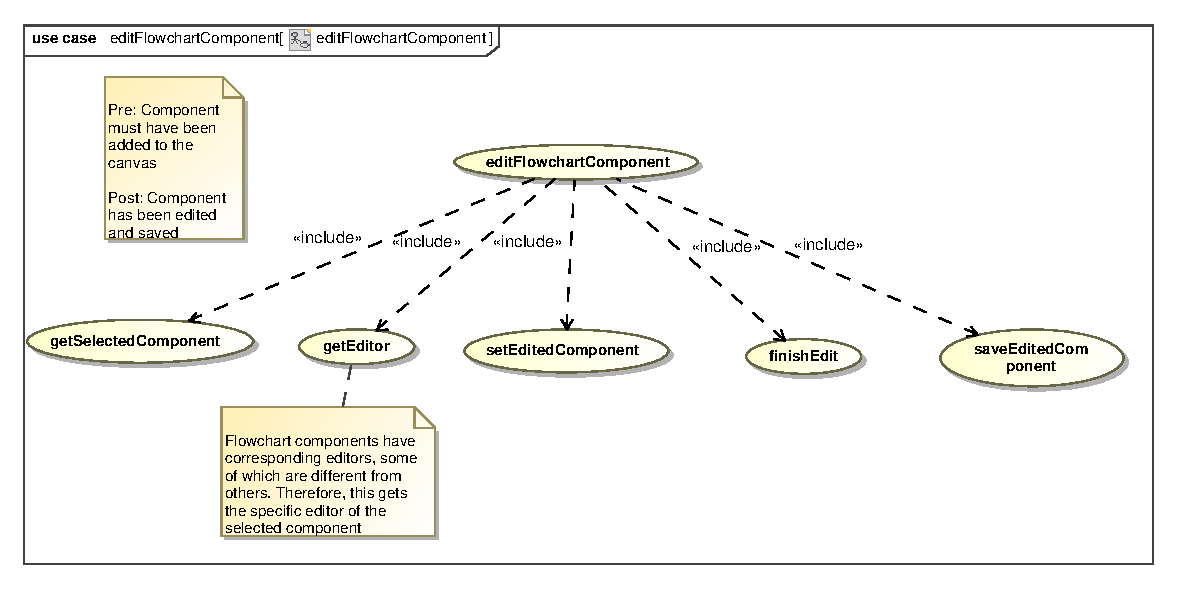
\includegraphics[width=500px]{editFlowchartComponent.eps}
\caption{editFlowchartComponent Use Case Diagram}
\end{figure}

\begin{figure}[H]
  \centering
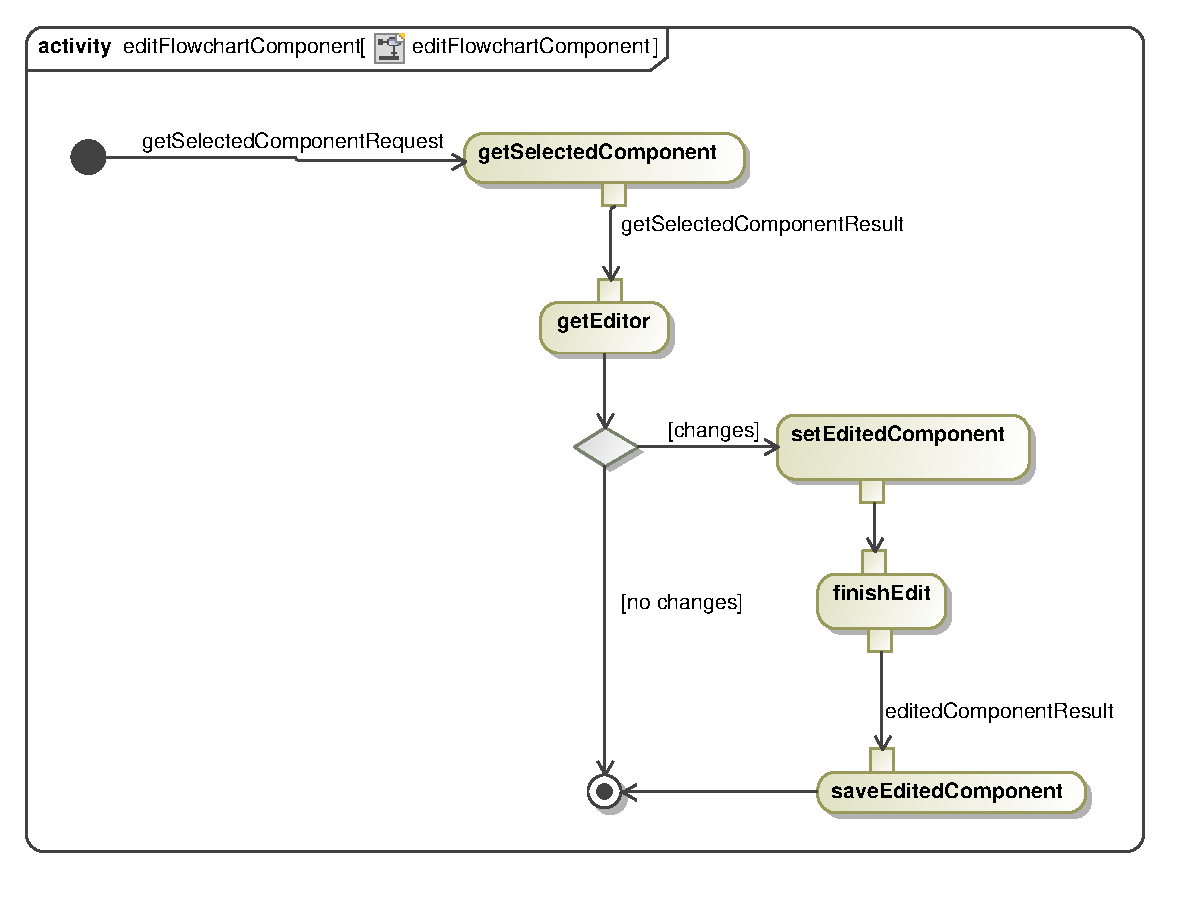
\includegraphics[width=500px]{editFlowchartComponentActivity.eps}
\caption{editFlowchartComponent Activity Diagram}
\end{figure}

\newpage
\subsection{deleteFlowchart}
The deleteFlowchartProject use case serves the purpose of removing a flowchart project.\newline\newline
\textbf{Pre Condition:} The flowchart to be deleted must exist\newline
\textbf{Pre Condition:} The flowchart to be deleted must be active\newline\newline
\textbf{Post Condition:} The flowchart must be removed from the workspace and a new flowchart must be active

\begin{figure}[H]
  \centering
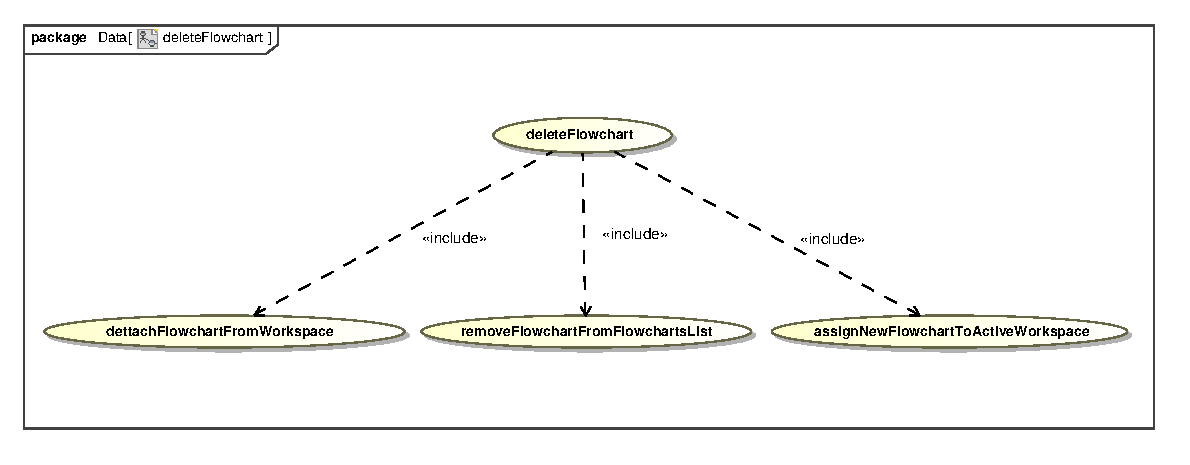
\includegraphics[width=500px]{deleteFlowchart.eps}
\caption{deleteFlowchart Use Case Diagram}
\end{figure}

\begin{figure}[H]
  \centering
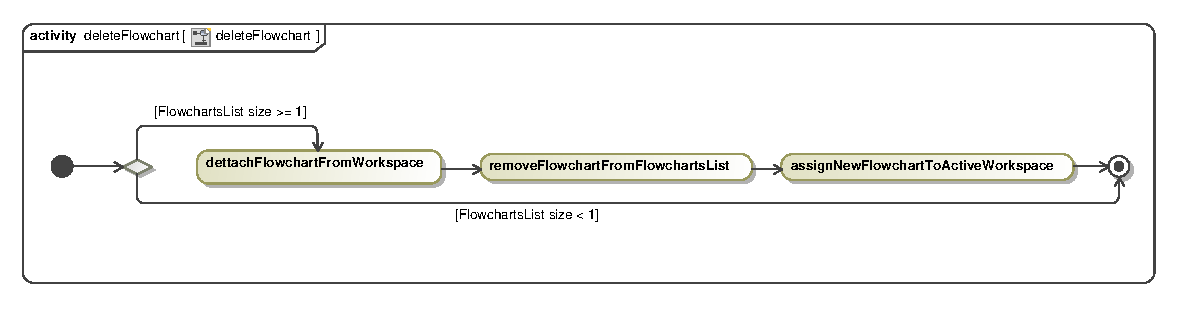
\includegraphics[width=500px]{deleteFlowchartActivity.eps}
\caption{deleteFlowchart Activity Diagram}
\end{figure}

\newpage
\subsection{saveFlowchart}
The saveFlowchart use case provides functionality for the user to save a flowchart.\newline\newline
\textbf{Pre Condition:} Canvas is open\newline\newline
\textbf{Post Condition:} Flowchart has been saved to file

\begin{figure}[H]
  \centering
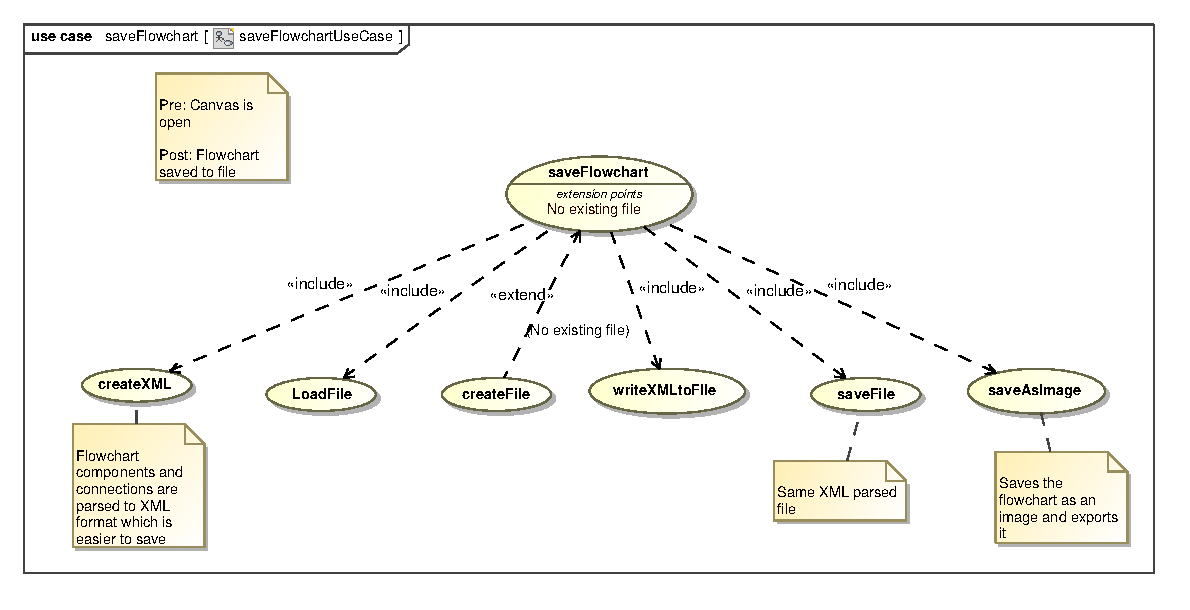
\includegraphics[width=500px]{saveFlowchartUseCase.eps}
\caption{saveFlowchart Use Case Diagram}
\end{figure}

\begin{figure}[H]
  \centering
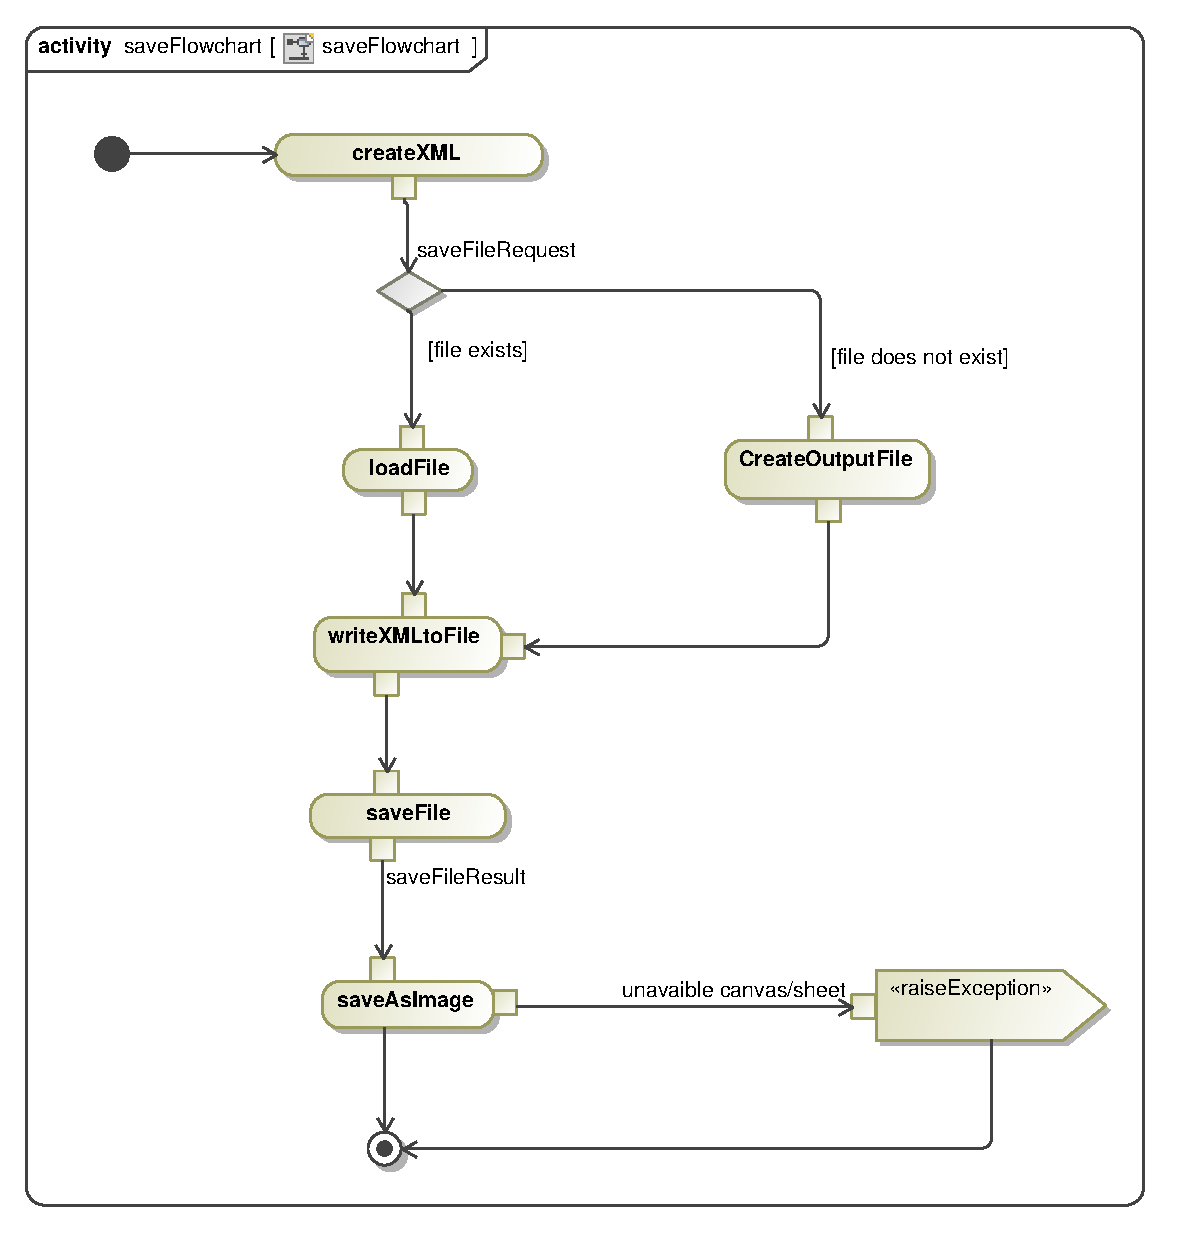
\includegraphics[width=500px]{saveFlowchart.eps}
\caption{saveFlowchart Activity Diagram}
\end{figure}

\newpage
\subsection{loadFlowchart}
loadFlowchart: users load flowcharts from existing files. The file is editable, can be modified by the user.\newline\newline
\textbf{Pre Condition:} File with correct extension already exists.\newline\newline
\textbf{Post Condition:} Open the file and make it editable in the canvas element.

\begin{figure}[H]
  \centering
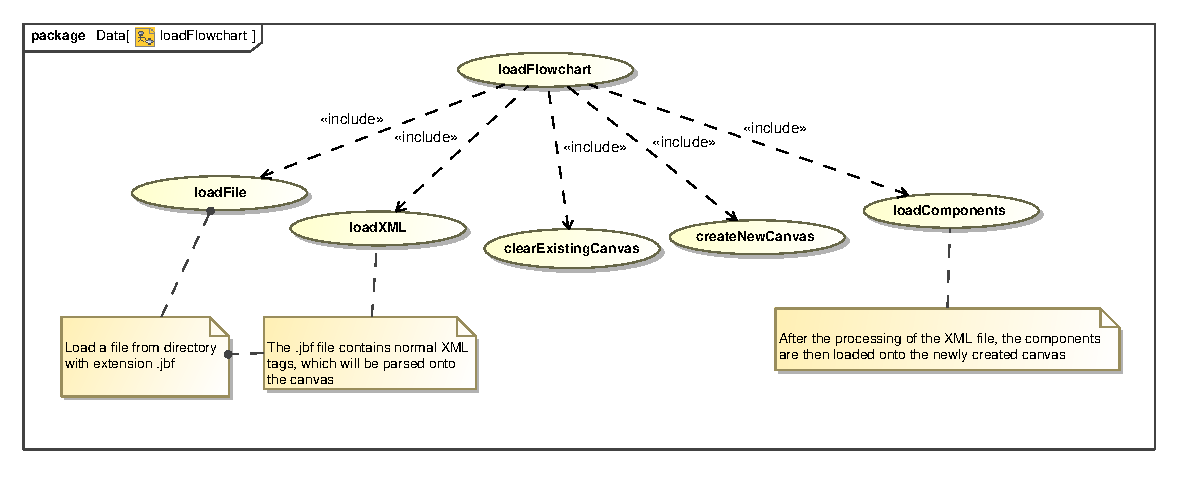
\includegraphics[width=500px]{loadFlowchart.eps}
\caption{loadFlowchart Use Case Diagram}
\end{figure}

\begin{figure}[H]
  \centering
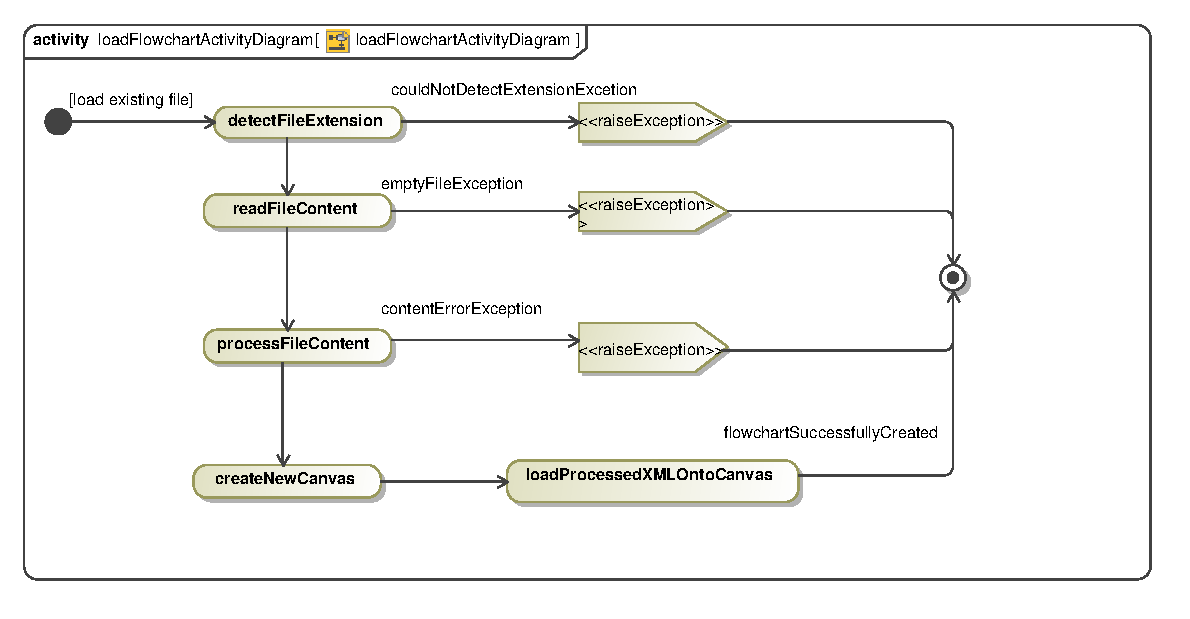
\includegraphics[width=500px]{loadFlowchartActivityDiagram.eps}
\caption{loadFlowchart Activity Diagram}
\end{figure}

\newpage
\subsection{deleteFlowchartComponent}
The deleteFlowchartComponent use case enables the functionality to delete individual components from the canvas.\newline\newline
\textbf{Pre Condition:} The canvas has to be available. Component exists in the canvas space and is in the components list.\newline\newline
\textbf{Post Condition:} The canvas is clear of any components that were selected for removal.

\begin{figure}[H]
  \centering
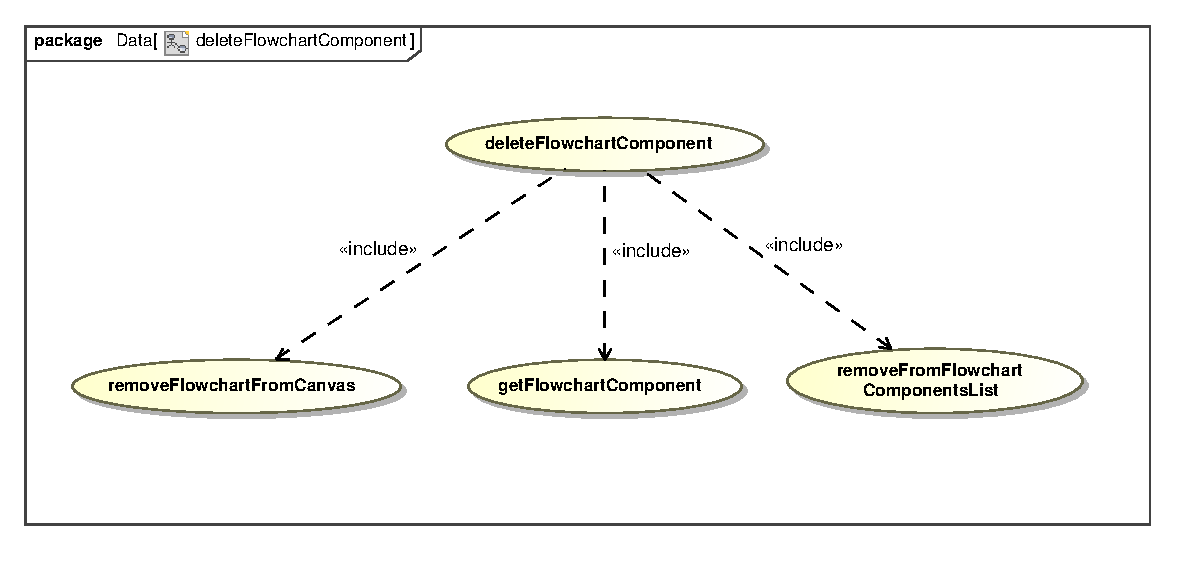
\includegraphics[width=500px]{deleteFlowchartComponentUseCase.eps}
\caption{loadFlowchart Use Case Diagram}
\end{figure}

\begin{figure}[H]
  \centering
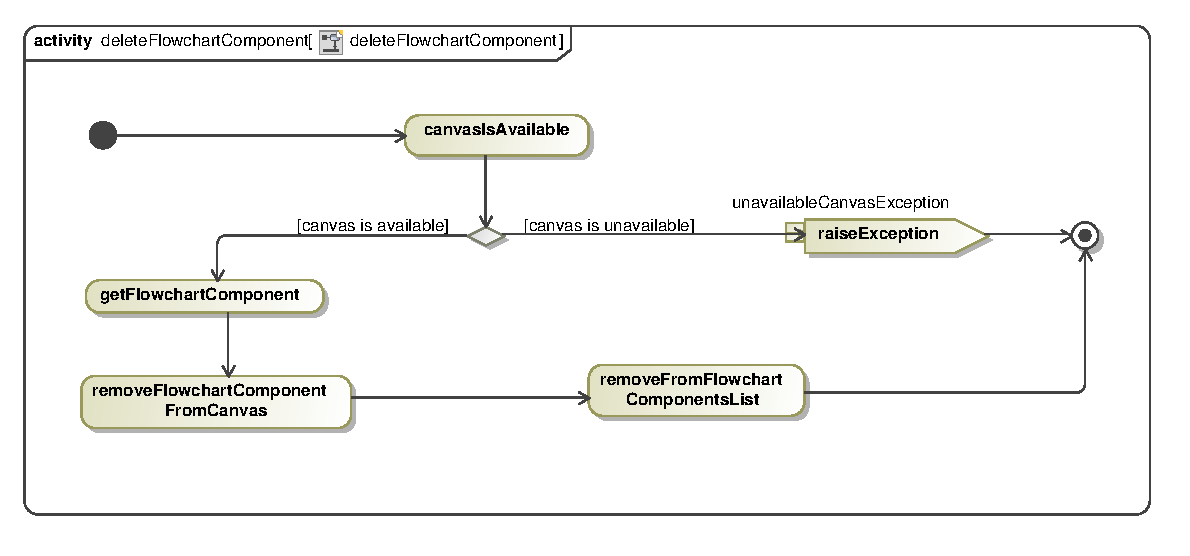
\includegraphics[width=500px]{deleteFlowchartComponentActivity.eps}
\caption{loadFlowchart Activity Diagram}
\end{figure}

\newpage
\subsection{runSimulationTool}
The runSimulation use case enables the functionality to execute the flowchart step-by-step or from start-to-end.\newline\newline
\textbf{Pre Condition:} Canvas has to be available.\newline\newline
\textbf{Post Condition:} Flowchart will return feedback of any errors, warnings or successful execution along with the results of any calculations.

\begin{figure}[H]
  \centering
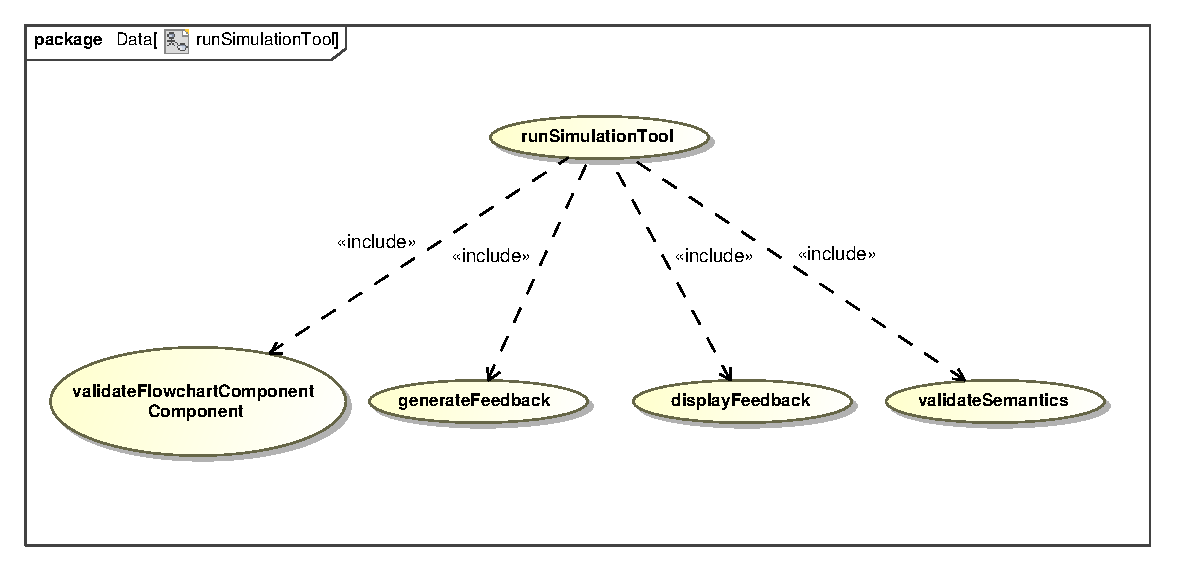
\includegraphics[width=500px]{runSimulationToolUseCase.eps}
\caption{loadFlowchart Use Case Diagram}
\end{figure}

\begin{figure}[H]
  \centering
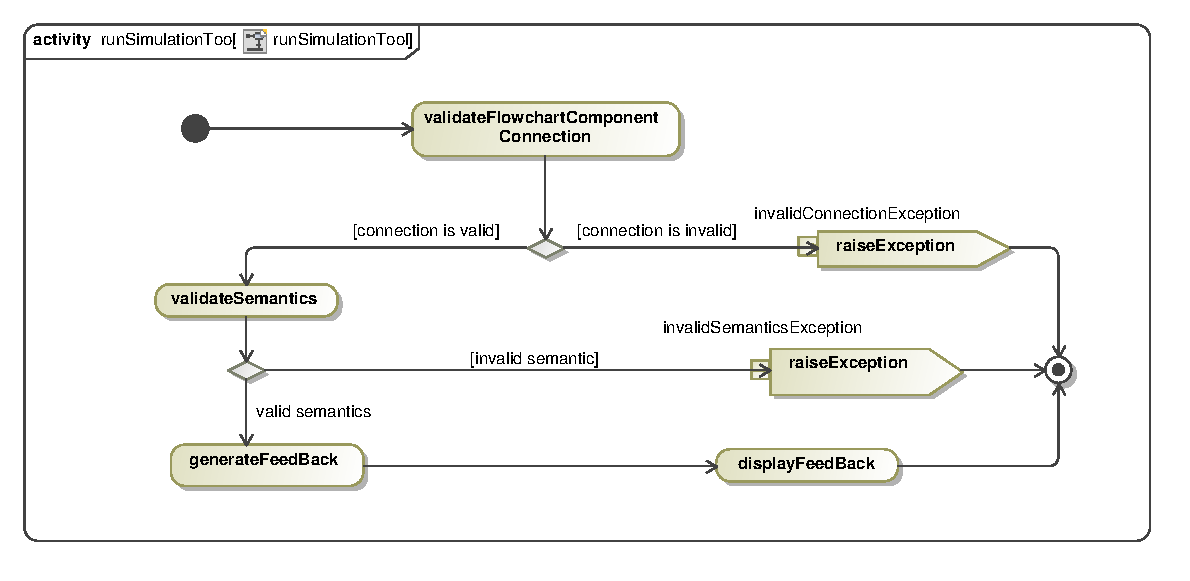
\includegraphics[width=500px]{runSimulationToolActivity.eps}
\caption{loadFlowchart Activity Diagram}
\end{figure}

\newpage
\section{The Domain Model - High-level}
\begin{figure}[H]
  \centering
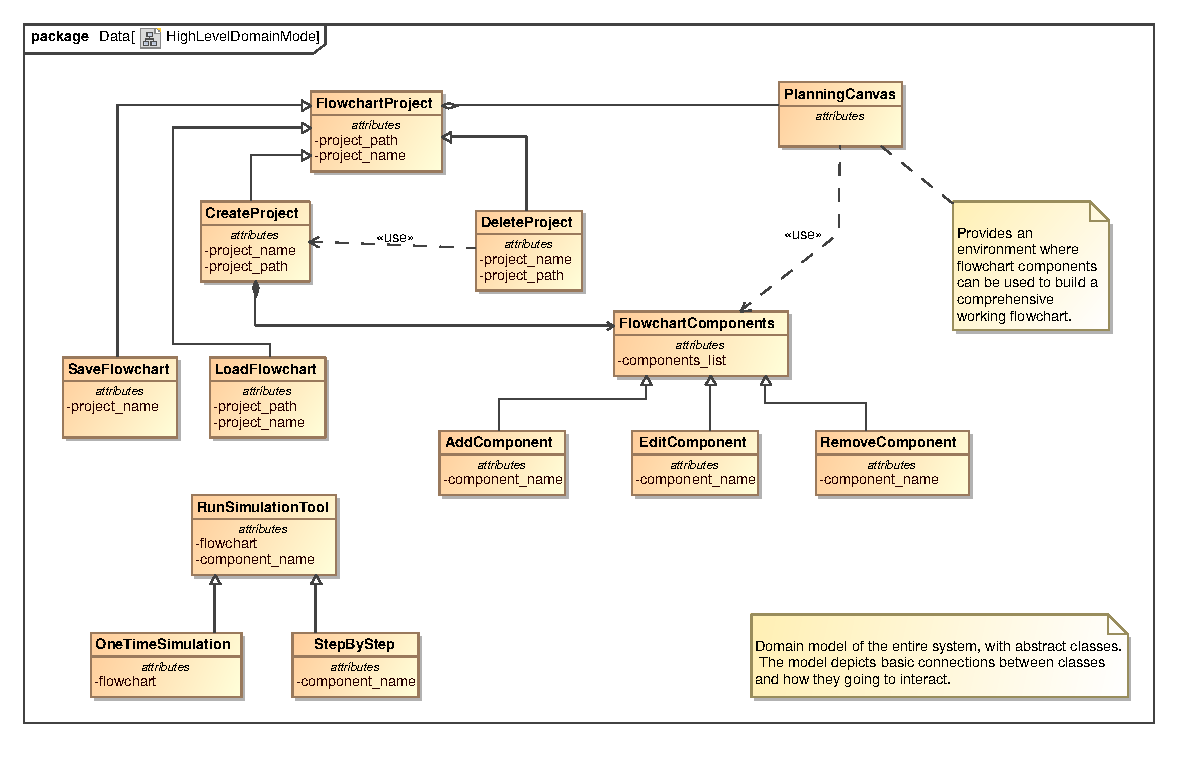
\includegraphics[width=500px]{HighLevelDomainModel.eps}
\caption{loadFlowchart Activity Diagram}
\end{figure}

\end{document}
